\documentclass[tikz,border=12pt]{standalone}
\usepackage[T1]{fontenc}
\usepackage{helvet}
\renewcommand{\familydefault}{\sfdefault}
\usepackage{amsmath}
\usetikzlibrary{arrows.meta, fit, backgrounds, positioning, calc, shapes.geometric}

% Semantic palette, shared across the method figures. Color encodes role:
%   blue   = BM25 / lexical step (none here)
%   red    = LLM step
%   amber  = document data and stores
%   green  = retrieved units and final output
%   gray   = query input
%   white  = agent tools (the action space)
\definecolor{queryfill}{HTML}{ECEFF2}
\definecolor{queryborder}{HTML}{8A96A3}
\definecolor{llmfill}{HTML}{F7E4E4}
\definecolor{llmborder}{HTML}{BE4F4F}
\definecolor{corpusfill}{HTML}{FBF0D5}
\definecolor{corpusborder}{HTML}{CFA23E}
\definecolor{outfill}{HTML}{E7F4E7}
\definecolor{outborder}{HTML}{59A05B}
\definecolor{regfill}{HTML}{F6F8FB}
\definecolor{regborder}{HTML}{C4CDD6}
\definecolor{darkline}{HTML}{333333}
\definecolor{subtext}{HTML}{5A5A5A}

\tikzset{
  card/.style={rectangle, rounded corners=5pt, align=center, draw=darkline,
               line width=0.8pt, minimum height=1.2cm, font=\small},
  query/.style={card, fill=queryfill, draw=queryborder, minimum width=2.0cm},
  llmproc/.style={card, fill=llmfill, draw=llmborder, minimum width=2.4cm},
  agentbox/.style={card, fill=llmfill, draw=llmborder, line width=1.0pt,
                   minimum width=3.0cm, minimum height=1.6cm},
  result/.style={card, fill=outfill, draw=outborder, minimum width=2.1cm},
  tool/.style={rectangle, rounded corners=3pt, draw=darkline, fill=white,
               line width=0.7pt, font=\ttfamily\scriptsize,
               minimum width=1.9cm, minimum height=0.64cm},
  db/.style={cylinder, shape border rotate=90, aspect=0.28, draw=corpusborder,
             fill=corpusfill, line width=0.8pt, minimum width=1.7cm,
             minimum height=1.0cm, font=\scriptsize, align=center, inner sep=1pt},
  region/.style={rounded corners=12pt, fill=regfill, draw=regborder, line width=0.8pt},
  toolgroup/.style={rounded corners=8pt, draw=regborder, dashed,
                    line width=0.85pt, fill=none},
  regtitle/.style={font=\small\bfseries, text=darkline},
  note/.style={font=\scriptsize\itshape, text=subtext, align=center},
  toolnote/.style={font=\scriptsize\itshape, text=subtext, align=left},
  flow/.style={-{Latex[length=2.2mm]}, line width=0.85pt, draw=darkline},
  feed/.style={-{Latex[length=1.9mm]}, line width=0.7pt, draw=corpusborder},
  act/.style={-{Latex[length=2.2mm]}, line width=0.9pt, draw=darkline},
  observe/.style={-{Latex[length=2.2mm]}, line width=0.9pt, draw=llmborder, dashed},
}

\def\dbdrop{1.0cm}

\begin{document}
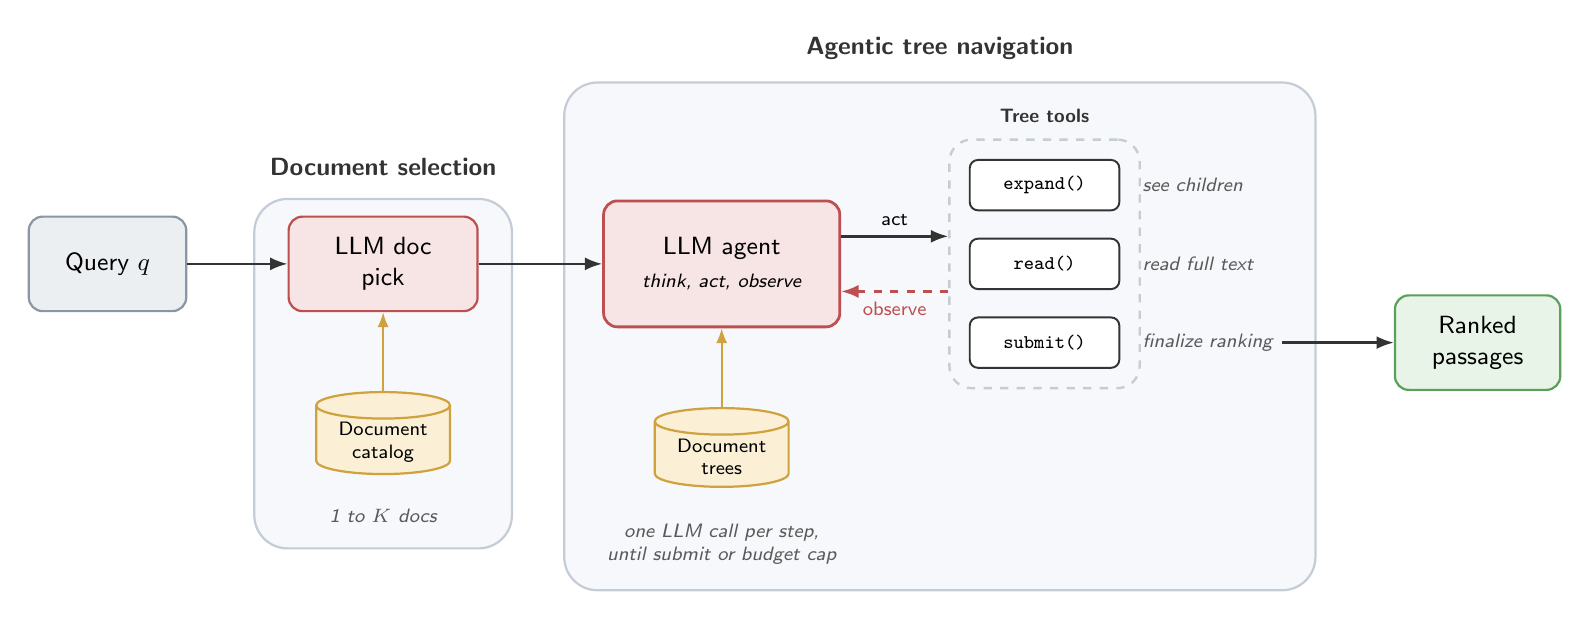
\begin{tikzpicture}

% Input (outside the phases)
\node[query] (query) at (-0.6,0) {Query $q$};

% Stage 1: LLM document selection
\node[llmproc] (pick) at (2.9,0) {LLM doc\\pick};
\node[db, below=\dbdrop of pick] (catalog) {Document\\catalog};

% Stage 2: agentic tree navigation. The agent reasons, calls a tool, observes
% the result, and repeats until it submits or hits the budget cap.
\node[agentbox] (agent) at (7.2,0) {LLM agent\\[1pt]{\scriptsize\itshape think, act, observe}};
\node[db, below=\dbdrop of agent] (trees) {Document\\trees};

% Tree tools, the agent's action space
\node[tool] (expand) at (11.3, 1.0) {expand()};
\node[tool] (read)   at (11.3, 0.0) {read()};
\node[tool] (submit) at (11.3,-1.0) {submit()};
\node[toolgroup, fit=(expand)(read)(submit), inner sep=7pt] (tools) {};
\node[font=\scriptsize\bfseries, text=darkline, anchor=south] (ttlabel)
  at ($(tools.north)+(0,0.08)$) {Tree tools};
\node[toolnote, right=0.16cm of expand] (en) {see children};
\node[toolnote, right=0.16cm of read]   (rn) {read full text};
\node[toolnote, right=0.16cm of submit] (sn) {finalize ranking};

% Output (outside the phases), aligned with submit() for a straight exit arrow
\node[result] (sources) at (16.8,-1.0) {Ranked\\passages};

% Notes
\node[note, below=0.30cm of catalog] (picknote) {1 to $K$ docs};
\node[note, below=0.34cm of trees] (agentnote)
  {one LLM call per step,\\until submit or budget cap};

% Flow
\draw[flow] (query) -- (pick.west);
\draw[feed] (catalog.north) -- (pick.south);
\draw[flow] (pick.east) -- (agent.west);
\draw[feed] (trees.north) -- (agent.south);

% The agentic loop: act out to the tools (top), observe the result back (bottom).
\draw[act] ([yshift=3.5mm]agent.east) -- ([yshift=3.5mm]tools.west)
  node[midway, above, font=\scriptsize] {act};
\draw[observe] ([yshift=-3.5mm]tools.west) -- ([yshift=-3.5mm]agent.east)
  node[midway, below, font=\scriptsize, text=llmborder] {observe};

% submit() finalizes (via its description) and exits straight to the output
\draw[flow] (sn.east) -- (sources.west);

% Phase panels. Input and output stay outside.
\begin{scope}[on background layer]
  \coordinate (bandB) at ($(trees.south)+(0,-0.14)$);
  \node[region, inner xsep=12pt, inner ysep=6pt,
        fit=(pick)(catalog)(picknote)(pick|-bandB)] (reg1) {};
  \node[region, inner xsep=12pt, inner ysep=6pt,
        fit=(agent)(trees)(agentnote)(tools)(ttlabel)(en)(rn)(sn)(agent|-bandB)] (reg2) {};
\end{scope}
\node[regtitle, anchor=south] at ($(reg1.north)+(0,0.16)$) {Document selection};
\node[regtitle, anchor=south] at ($(reg2.north)+(0,0.16)$) {Agentic tree navigation};

\end{tikzpicture}
\end{document}
